% !TEX TS-program = xeLaTeX+MakeIndex+BibTeX 
\documentclass[11pt,compress,xcolor=x11names,UTF8]{ctexbeamer}
\usepackage{xeCJK}
\setCJKsansfont[BoldFont={Source Han Sans CN},ItalicFont={Source Han Sans CN}]{Source Han Sans CN} 
\setsansfont{DejaVu Sans} 

\usetheme{Darmstadt}
\useoutertheme[subsection=false,footline=empty]{miniframes}
\usecolortheme{seahorse}
\usecolortheme[named=SpringGreen4]{structure}
\useinnertheme{rectangles} % default circles rectangles rounded

\setbeamertemplate{caption}[numbered] % 序号
\setbeamercovered{transparent=15}
\setbeamersize{text margin left=0.6cm, text margin right=0.6cm} % 设置页边距

\usepackage{ragged2e}
\renewcommand{\raggedright}{\leftskip=0pt \rightskip=0pt plus 0cm} % 对齐
\usepackage{natbib} % 参考文献
\graphicspath{{figure/}} % 图片路径

\title{空间广义线性混合模型及其在预测流行病中的应用}
\subtitle{Spatial Generalized Linear Mixed Models with Application to Prevalence Mapping}

\author{黄湘云\and 李再兴}

\institute[CUMTB]{理学院\\ 中国矿业大学(北京)}
\date{2018年5月}

\titlegraphic{
\includegraphics[height=0.15\textwidth]{figure/cumtb}}

\subject{毕业答辩}
\keywords{数据分析、统计计算}

\begin{document}
\raggedright

\maketitle



\begin{frame}
  \frametitle{内容提要}
  \tableofcontents  
\end{frame}


\section{引言}


\subsection{研究意义}

\begin{frame}{Examples}

\begin{enumerate}
\item radionuclide concentrations on Rongelap Island
\item childhood malaria in the gambia
\item Loa loa prevalence in Cameroon and surrounding areas
\end{enumerate}

\end{frame}

\begin{frame}{Introduction}
\citet{Diggle2002}
\begin{itemize}
\item the effects of child level covariates (age and bed net use)
\item village level covariates (the primary health care and greenness of surrounding vegetation)
\item separate components for residual spatial
\item non-spatial extrabinomial variation
\end{itemize}
$\mathbb{R}^{n}$
$$ \log \{p_{ij}/(1-p_{ij})\} =\alpha + \beta'z_{ij} + U_{i} + S(x_{i})$$

\end{frame}

\subsection{文献综述}

\subsection{主要内容}


\section{模型(SGLMM)}

\subsection{模型结构}

\subsection{计算方法}

\subsection{数据分析}

\section{结论与展望}



\begin{frame}{疟疾流行度与植被关系}
\begin{figure}
\centering
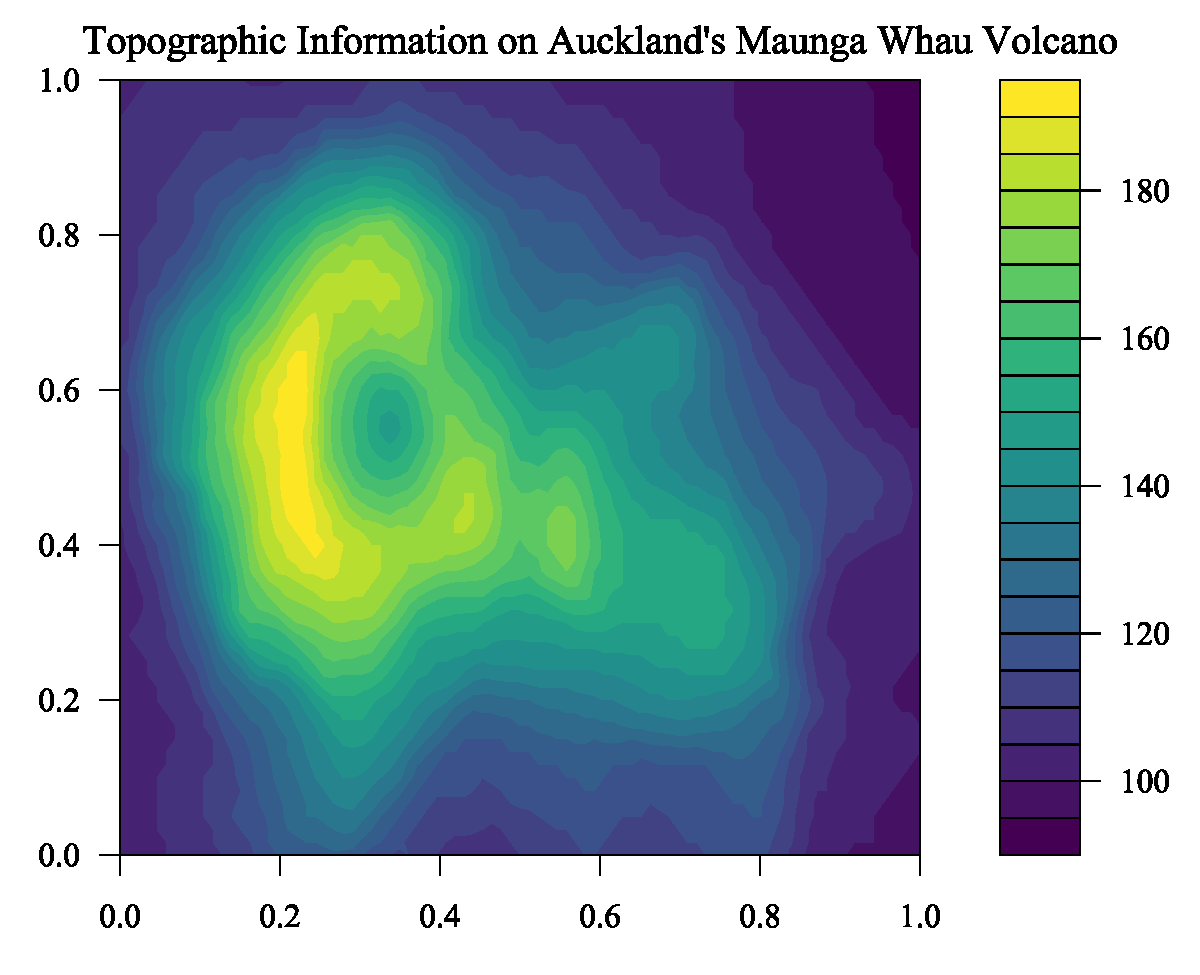
\includegraphics[width=.75\textwidth]{volcano02}
\end{figure}
\end{frame}

\begin{frame}{疟疾流行度与植被关系}
\begin{figure}
\centering
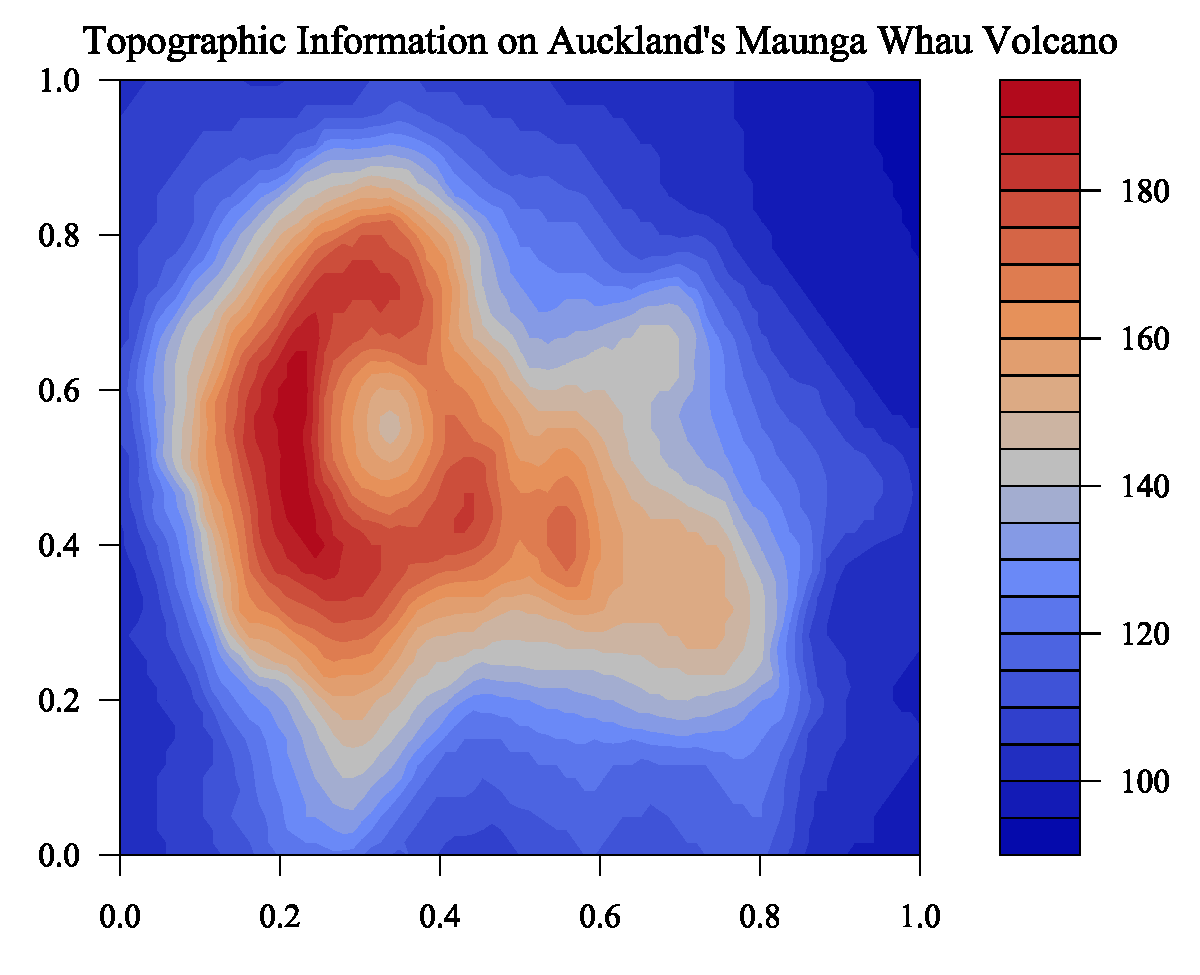
\includegraphics[width=.8\textwidth]{volcano03}
\end{figure}
\end{frame}



\begin{frame}

  \centerline{\Huge\color{red} 谢谢! }

\end{frame}



\begin{frame}[allowframebreaks]
\frametitle{参考文献}
% pkgs <- c("nlme","lme4","geoR","geoRglm","PrevMap","INLA","spatial")
% write_bib(pkgs, file = "R-GLMM-pkgs.bib")
\bibliographystyle{authordate1}
\bibliography{R-GLMM-pkgs}
\end{frame}

\end{document} 